\documentclass[border=6pt]{standalone}
\usepackage{tikz}
\usetikzlibrary{arrows.meta,positioning,calc}
\begin{document}
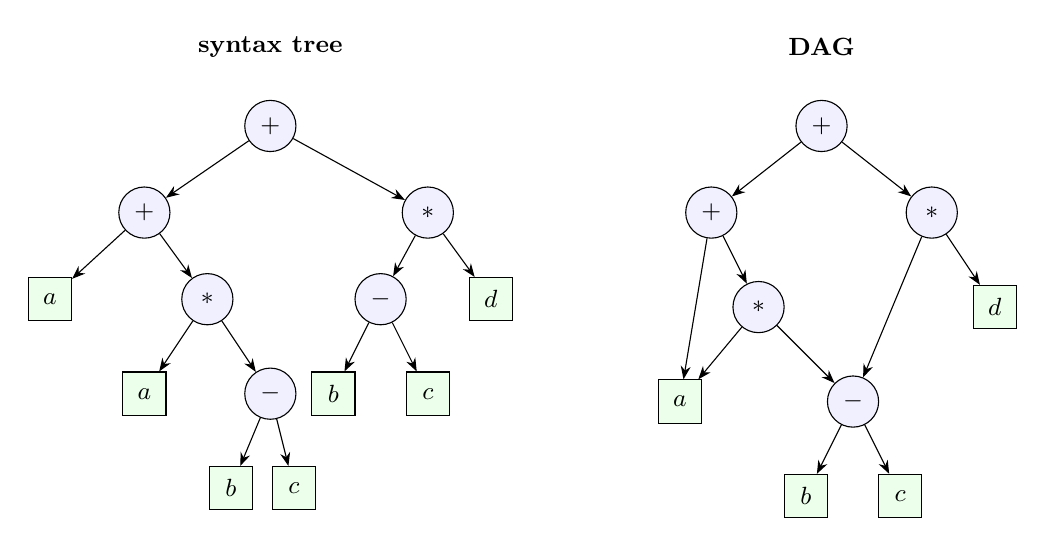
\begin{tikzpicture}[>=Stealth,font=\small,
 op/.style={draw,circle,minimum size=0.65cm,inner sep=0pt,fill=blue!6},
 lf/.style={draw,rectangle,minimum size=0.55cm,inner sep=0pt,fill=green!8,font=\small}]
% syntax tree
\node[font=\small\bfseries] at (2.4,0.6) {syntax tree};
\node[op] (t1) at (2.4,-0.4) {$+$};
\node[op] (t2) at (0.8,-1.5) {$+$};
\node[op] (t3) at (4.4,-1.5) {$*$};
\node[lf] (ta1) at (-0.4,-2.6) {$a$};
\node[op] (t4) at (1.6,-2.6) {$*$};
\node[op] (t5) at (3.8,-2.6) {$-$};
\node[lf] (td) at (5.2,-2.6) {$d$};
\node[lf] (ta2) at (0.8,-3.8) {$a$};
\node[op] (t6) at (2.4,-3.8) {$-$};
\node[lf] (tb1) at (3.2,-3.8) {$b$};
\node[lf] (tc1) at (4.4,-3.8) {$c$};
\node[lf] (tb2) at (1.9,-5.0) {$b$};
\node[lf] (tc2) at (2.7,-5.0) {$c$};
\draw[->] (t1)--(t2); \draw[->] (t1)--(t3);
\draw[->] (t2)--(ta1); \draw[->] (t2)--(t4);
\draw[->] (t3)--(t5); \draw[->] (t3)--(td);
\draw[->] (t4)--(ta2); \draw[->] (t4)--(t6);
\draw[->] (t6)--(tb2); \draw[->] (t6)--(tc2);
\draw[->] (t5)--(tb1); \draw[->] (t5)--(tc1);
% DAG
\node[font=\small\bfseries] at (9.4,0.6) {DAG};
\node[op] (d1) at (9.4,-0.4) {$+$};
\node[op] (d2) at (8.0,-1.5) {$+$};
\node[op] (d3) at (10.8,-1.5) {$*$};
\node[op] (d4) at (8.6,-2.7) {$*$};
\node[lf] (dd) at (11.6,-2.7) {$d$};
\node[op] (d5) at (9.8,-3.9) {$-$};
\node[lf] (da) at (7.6,-3.9) {$a$};
\node[lf] (db) at (9.2,-5.1) {$b$};
\node[lf] (dc) at (10.4,-5.1) {$c$};
\draw[->] (d1)--(d2); \draw[->] (d1)--(d3);
\draw[->] (d2)--(da); \draw[->] (d2)--(d4);
\draw[->] (d3)--(d5); \draw[->] (d3)--(dd);
\draw[->] (d4)--(da); \draw[->] (d4)--(d5);
\draw[->] (d5)--(db); \draw[->] (d5)--(dc);
\end{tikzpicture}
\end{document}
